%%=============================================================================
%% Asimov = median of toy pseudo-experiments -- histogram checks
%%
%% HWW meeting -- 22/07/2026.  Marta Silva.
%%
%% Build:  make          (lualatex through latexmk, cvmfs texlive)
%% Theme:  ../beamer/beamerthememarta.sty
%%
%% Scope for this meeting (2026-07-21): histogram analysis only, NSBI parked.
%% Goal is a discussion, not a result talk -- the two "Ask" slides carry the
%% actual questions for the supervisor. Nothing on them is asserted as
%% settled; they are proposals to react to.
%%
%% Content provenance:
%%   * process, yields                          -- docs/context.md
%%   * the toys and the statistic t(mu)          -- notebooks/histogram_reproduction.ipynb §1
%%   * the two numbers on the "curves vs quantiles" slide (0.455, 1.185) are
%%     properties of the noncentral chi-square distribution, derived in
%%     notebooks/histogram_reproduction.ipynb §2 -- not measured, not in
%%     dispute on their own; what's open is whether this is the right thing
%%     to be testing, which is the ask itself.
%%
%% The histogram-results slide is a placeholder: it waits on the
%% verification walkthrough (Plan Step 1) and the reworked figures
%% (scripts/make_talk_figures.py, Plan Step 2).
%%=============================================================================
\documentclass[aspectratio=169, 11pt]{beamer}

\usetheme[accent=AD1A72]{marta}
\martaset{
  author = Marta Silva,
  venue  = HWW meeting,
  date   = 22/07/2026,
}

\usepackage{tikz-feynman}
\tikzfeynmanset{compat=1.1.0}

\graphicspath{{figures/}{../../../output/talk-figs/}}

\title{Asimov = median of toy pseudo-experiments}
\subtitle{Checks for the histogram analysis}
\author{Marta Silva}
\date{HWW meeting \textemdash{} 22 July 2026}

%%--------------------------------------------------------------- shorthands ---
\newcommand{\mfl}{m_{4\ell}}
\newcommand{\mutrue}{\mu_{\mathrm{true}}}
\newcommand{\muhat}{\hat\mu}
\newcommand{\fb}{\,\mathrm{fb}^{-1}}

%%----------------------------------------------------------- Feynman diagrams --
\newcommand{\signaldiagram}{%
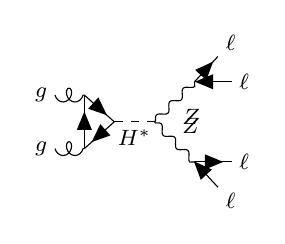
\begin{tikzpicture}
  \footnotesize
  \begin{feynman}
    \vertex (g1) {\(g\)};
    \vertex[below=0.68cm of g1] (g2) {\(g\)};
    \vertex[right=0.55cm of g1] (t1);
    \vertex[right=0.55cm of g2] (t2);
    \vertex[right=0.38cm of t1, yshift=-0.34cm] (t3);
    \vertex[right=0.51cm of t3] (h);
    \vertex[above right=0.72cm of h] (z1);
    \vertex[below right=0.72cm of h] (z2);
    \vertex[above right=0.42cm of z1] (l1) {\(\ell\)};
    \vertex[right=0.47cm of z1] (l2) {\(\ell\)};
    \vertex[right=0.47cm of z2] (l3) {\(\ell\)};
    \vertex[below right=0.42cm of z2] (l4) {\(\ell\)};
    \diagram* {
      (g1) -- [gluon] (t1),
      (g2) -- [gluon] (t2),
      (t1) -- [fermion] (t3) -- [fermion] (t2) -- [fermion] (t1),
      (t3) -- [scalar, edge label'=\(H^{*}\)] (h),
      (h) -- [boson, edge label'=\(Z\)] (z1),
      (h) -- [boson, edge label=\(Z\)] (z2),
      (z1) -- [fermion] (l1),
      (z1) -- [anti fermion] (l2),
      (z2) -- [fermion] (l3),
      (z2) -- [anti fermion] (l4),
    };
  \end{feynman}
\end{tikzpicture}%
}
\newcommand{\bkgdiagram}{%
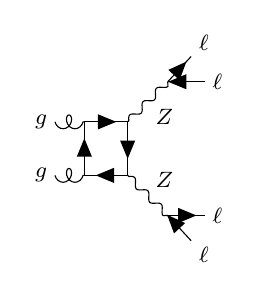
\begin{tikzpicture}
  \footnotesize
  \begin{feynman}
    \vertex (g1) {\(g\)};
    \vertex[below=0.68cm of g1] (g2) {\(g\)};
    \vertex[right=0.55cm of g1] (b1);
    \vertex[right=0.55cm of g2] (b2);
    \vertex[right=0.55cm of b1] (b3);
    \vertex[right=0.55cm of b2] (b4);
    \vertex[above right=0.72cm of b3] (z1);
    \vertex[below right=0.72cm of b4] (z2);
    \vertex[above right=0.42cm of z1] (l1) {\(\ell\)};
    \vertex[right=0.47cm of z1] (l2) {\(\ell\)};
    \vertex[right=0.47cm of z2] (l3) {\(\ell\)};
    \vertex[below right=0.42cm of z2] (l4) {\(\ell\)};
    \diagram* {
      (g1) -- [gluon] (b1),
      (g2) -- [gluon] (b2),
      (b1) -- [fermion] (b3) -- [fermion] (b4) -- [fermion] (b2) -- [fermion] (b1),
      (b3) -- [boson, edge label'=\(Z\)] (z1),
      (b4) -- [boson, edge label=\(Z\)] (z2),
      (z1) -- [fermion] (l1),
      (z1) -- [anti fermion] (l2),
      (z2) -- [fermion] (l3),
      (z2) -- [anti fermion] (l4),
    };
  \end{feynman}
\end{tikzpicture}%
}

\begin{document}

%%------------------------------------------------------------------ title -----
\begin{frame}[plain, noframenumbering]
  \titlepage
\end{frame}

%%========================================================= 1 the question =====
\begin{frame}{The question}
  \msg{Does the no-fluctuation dataset actually tell us what a real experiment will see?}

  \begin{itemize}\small
    \item To know how sensitive an analysis will be, we normally fit one fake dataset where
      nothing fluctuates \textemdash{} the \alert{Asimov dataset}.
    \item That's supposed to stand in for running thousands of toy pseudo-experiments and taking
      the median. Much cheaper, if it's true.
    \item The catch: that substitution is a \alert{large-sample} result. Off-shell Higgs at
      $1\fb$ is about six events \textemdash{} not obviously a large sample.
    \item So before trusting it for anything fancier, we wanted to actually check it, carefully,
      for the simplest analysis we have: a plain histogram fit.
  \end{itemize}

  \takeaway{This is a check, not a result talk. A lot of it is us thinking out loud about whether
  we're even testing the right thing.}
\end{frame}

%%============================================================ 2 the process ===
\begin{frame}{The process}
  \msg{Off-shell $gg \to H^{*} \to ZZ \to 4\ell$, at parton level.}

  We can get to $4\ell$ two ways: through the Higgs, or not at all. Same final state, so they
  interfere.

  \vspace{-0.35cm}
  \centering
  \begin{columns}[c, onlytextwidth]
    \begin{column}{0.5\textwidth}
      \centering
      \signaldiagram\\[0.05cm]
      \footnotesize\textbf{signal}
    \end{column}
    \begin{column}{0.5\textwidth}
      \centering
      \bkgdiagram\\[0.05cm]
      \footnotesize\textbf{background}
    \end{column}
  \end{columns}
  \raggedright

  \takeaway{Signal and background aren't separable event by event \textemdash{} the interference
  term is part of what any fit has to deal with, histogram or not.}
\end{frame}

%%============================================================ 3 the setup =====
\begin{frame}{The setup}
  \msg{One parameter, one histogram, lots of toys.}

  \begin{columns}[T, onlytextwidth]
    \begin{column}{0.55\textwidth}
      \begin{itemize}\small
        \item Every event carries its matrix elements, so we can reweight it to any signal
          strength $\mu$ exactly \textemdash{} no detector simulation.
        \item Fit parameter: just $\mu$. No nuisance parameters here.
        \item For a toy, we let every event weight fluctuate on its own (Poisson noise) and refit.
          2000 toys per luminosity point, generated at $\mutrue = 1$.
        \item $\mu$ scanned over $[0,4]$; luminosities from $1$ to $3000\fb$.
      \end{itemize}
    \end{column}
    \begin{column}{0.41\textwidth}
      \footnotesize
      \textbf{Expected events at $\mu = 1$}
      \vspace{0.15cm}

      \begin{tabular}{@{}l@{\hskip 0.7em}r@{\hskip 0.7em}r@{\hskip 0.7em}r@{}}
        \hline
                     & $1\fb$  & $100\fb$ & $1000\fb$ \\
        \hline
        signal       & $0.31$  & $31.0$   & $309.9$ \\
        background   & $5.95$  & $595.3$  & $5953.0$ \\
        interference & $-0.61$ & $-60.6$  & $-606.4$ \\
        \hline
        total        & $5.66$  & $565.7$  & $5656.5$ \\
        \hline
      \end{tabular}

      \vspace{0.1cm}
      At $1\fb$ the whole experiment is \num{six events} \textemdash{} the signal is a third of
      one of them.
    \end{column}
  \end{columns}

  \takeaway{Small numbers. Worth keeping in mind for everything that follows.}
\end{frame}

%%============================================================== 4 ask one =====
\begin{frame}{Ask 1: subtract each toy's own minimum first?}
  \msg{What we compare, before we compare it.}

  \begin{itemize}\small
    \item Right now, before comparing a toy to Asimov, we shift the toy's whole curve down by
      its \emph{own} best fit: we look at $t(\mu) = -2\ln L(\mu) - \big(-2\ln L(\muhat)\big)$,
      not the raw $-2\ln L(\mu)$.
    \item The reasoning: each toy's curve sits at a random overall height that has nothing to do
      with $\mu$ \textemdash{} it's just how lucky that particular toy got. Subtracting the
      minimum removes that.
    \item Tae's original slides didn't do this \textemdash{} they took the median of the raw
      curves directly, offset and all.
  \end{itemize}

  \ask{Is subtracting each toy's own minimum the right move, or is there a reason to compare the
  raw curves instead?}
\end{frame}

%%============================================================== 5 ask two =====
\begin{frame}{Ask 2: should the curves match, or just the quantiles?}
  \msg{Even after that subtraction, we're not sure ``Asimov = median'' is the right target.}

  \begin{itemize}\small
    \item Our rough back-of-envelope guess, if the usual large-sample assumptions hold: the
      \emph{median} toy curve shouldn't sit exactly on the Asimov curve \textemdash{} it should
      sit a bit above it near $\mutrue$, and be a bit wider, just from basic $\chi^2$ statistics.
    \item If that's right, then maybe ``Asimov = median of toys'' was never quite the thing to
      check curve-by-curve. Maybe what should actually line up is the \emph{spread} of toy
      curves at each $\mu$ \textemdash{} the $16\%/50\%/84\%$ quantiles \textemdash{} against
      what Asimov predicts for that spread.
    \item We haven't fully convinced ourselves this is the right framing.
  \end{itemize}

  \ask{Should we be checking curve-on-curve agreement, or agreement of the quantiles at each
  $\mu$? Is there a convention you'd expect us to use here?}
\end{frame}

%%========================================================= 6 histogram result =
\todoframe{%
  Waits on the verification walkthrough and the reworked figures
  (\texttt{scripts/make\_talk\_figures.py}). Content: the measured toy spread against what Asimov
  predicts, at a few luminosities, plus an honest read of where it lines up and where it doesn't.%
}{Histogram results}

%%------------------------------------------------------------------ backup ----
\backupdivider

\end{document}
